\chapter*{Le langage SQL}
\setcounter{chapter}{1}
\setcounter{Exercise}{0}
Dans le chapitre précédent, nous avons vu les bases de données d'un point de vue théorique avec le modèle relationnel.

En pratique, les bases de données sont stockées sur les ordinateurs, il faut donc des logiciels qui permettent de créer, utiliser et maintenir des bases de données relationnelles.
On parle des \motcle{systèmes de gestion de bases de données relationnelles (SGBDR)}.

Pratiquement tous les systèmes relationnels utilisent le langage \motcle{SQL} pour interroger les bases de données. 
Les instructions SQL s’écrivent d’une manière qui ressemble à celle de phrases ordinaires en anglais. 
On appelle ces phrases des~\motcle{requêtes}, elles seront exécutées pour effectuer une action spécifique : sélectionner des données, supprimer des données, ajouter des données, mettre à jour des données...

C’est un langage déclaratif, c’est-à-dire qu’il permet de décrire le résultat escompté, sans décrire la manière de l’obtenir (le SGBD s'occupe de tout).

\begin{Astuce} 
    Le langage SQL n’est pas sensible à la casse, mais on a l’habitude d’écrire les instructions en majuscules, on peut écrire les instructions sur plusieurs lignes avec ou sans indentation et chaque instruction doit être terminée par un point-virgule.
\end{Astuce}

Nous verrons cette année les instructions de manipulation du contenu de la base de données qui commencent par les mots clés :
\begin{description}
    \item[CREATE]: Créer des tables
    \item[DROP]: Supprimer des tables
    \item[SELECT]: Sélectionner des données
    \item[UPDATE]: Modifier des données
    \item[INSERT]: Insérer des données
    \item[DELETE]: Supprimer des données.
\end{description}

\begin{Astuce}
    En SQL, le symbole /* et */ permettent de faire des commentaires qui peuvent s'étendre sur plusieurs lignes (multiligne).
    Le commentaire multiligne a l’avantage de pouvoir indiquer où commence et où se termine le commentaire. Il est donc possible de l’utiliser en plein milieu d’une requête SQL sans problème.
\begin{lstlisting}[style=SQLstyle, language=SQL]
    /* mon
    commentaire
    multi-ligne */
\end{lstlisting}
\end{Astuce}

\section{Créer des tables}
Pour créer des tables (relation) on utilise CREATE TABLE, il nous faut préciser le nom de la table, le nom des attributs, leurs types, d'éventuelle clé primaire et d'éventuelle clé étrangère en indiquant bien sur la clé primaire de référence. 
Voici la syntaxe à suivre :
\begin{lstlisting}[style=SQLstyle, language=SQL]
    CREATE TABLE table_name ( /* On crée la table en choississant son nom */
    id INT NOT NULL,          /* On crée un attribut id de type INT qui ne pourra pas être laissé vide */
    foreignId INT NOT NULL,   /* On crée un attribut foreignId de type INT qui ne pourra pas être laissé vide */
    col1 INT,                 /* On crée un attribut col1 de type INT qui pourra être laissé vide */
    col2 TEXT,                /* On crée un attribut col2 de type TEXT qui pourra être laissé vide */
    PRIMARY KEY (id),         /* On déclare id comme un clé primaire de la table */
    FOREIGN KEY (foreignId) REFERENCES table2(id) /* On déclare foreignId comme une clé étrangère de la table, qui se réfère à la clé primaire id de la table2 */
); 
\end{lstlisting}

\vfill

\begin{Exercise}
    En reprenant le modèle relationnel de SQL mystery.
    \Question donner la requête permettant de créer la table drivers\_license\\
    \emptybox{6cm}
    \vfill
    \Question donner la requête permettant de créer la table person\\
    \emptybox{6cm}
\end{Exercise} 

\vfill

\section{Supprimer des tables}
Si l'on peut créer des tables, on peut aussi en supprimer, pour cela, on utilise DROP TABLE :
\begin{lstlisting}[style=SQLstyle, language=SQL]
DROP TABLE table_name;
\end{lstlisting}

\begin{Exercise}
    En reprenant le modèle relationnel de SQL mystery.
    \Question donner la requête permettant de supprimer table drivers\_license.\\
    \emptybox{4cm}
\end{Exercise} 

\vfill

\section{Insérer des données}
Bien sûr, on va aussi vouloir ajouter des données dans nos tables.
Il nous faudra préciser la table et les valeurs à ajouter.
Pour cela, on utilise INSERT INTO :
\begin{lstlisting}[style=SQLstyle, language=SQL]
INSERT INTO table_name /* On selectionne la table table_name */
(col1, col2, ...)      /* On précise les attributs */
 VALUES                /* Et maintenant les valeurs */
(val1e1, val2e1 ...), /* On ajoute un nouvel enregistrement */
(val1e2, val2e2 ...), /* puis un autre */
(val1e3, val2e3 ...); /* et un dernier */
\end{lstlisting}

\vfill

\begin{Exercise}
    \begin{center}\begin{tabular}{|c c|}
    \hline
    \multicolumn{2}{|c|}{\textbf{interview}} \\
    \hline
        person\_id & transcript \\
        \hline
        \hline
        10007	& "à 9h j'étais déjà parti au travail" \\
        54263 & "j'ai entendu un cri effroyable"  \\
    \hline
    \end{tabular}
    \end{center}
    
    \Question donner la requête permettant d'ajouter les éléments du tableau ci-dessus à la table interview.\\    

    \emptybox{5cm}
\end{Exercise} 

\newpage

\section{Sélectionner les données}
Une des fonctionnalités les plus importantes des SGBD est la sélection des données, bien sûr, on va vouloir sélectionner les données selon des conditions, pour filtrer qu'une partie des données pertinentes.

Les requêtes de sélection sont parmi les plus fréquemment appeler, par exemple, dès que vous vous connectez à votre compte, il faut charger votre nom, votre prénom... il faut donc une requête de sélection.

De plus, les requêtes de sélection permettent également de fouiller les données, pour extraire des caractéristiques importantes.
C'est elle que nous utiliserons pour résoudre l'enquête dans SQL Murder Mystery.

\begin{lstlisting}[style=SQLstyle, language=SQL]
SELECT col1, col2
FROM table_name
WHERE condition;
\end{lstlisting}

SELECT veut dire "sélectionner" en anglais, FROM veut dire "depuis" en anglais et WHERE veut dire "où" en anglais (Attention à l'accent, le "où" ici est de position).

Pour sélectionner toutes les colonnes, on utilise le symbole *.
\begin{lstlisting}[style=SQLstyle, language=SQL]
SELECT * 
FROM table_name
WHERE condition;
\end{lstlisting}

On peut aussi sélectionner une colonne, mais décider de changer son nom dans le tableau retourner, pour cela, on utilise AS.
\begin{lstlisting}[style=SQLstyle, language=SQL]
SELECT col1 AS nom1, col2
FROM table_name
WHERE condition;
\end{lstlisting}


Nous l'avons vu, on va vouloir sélectionner selon des conditions, voici quelques exemples d'opérateur utile pour ces conditions :
\begin{description}
    \item [Les opérateurs classiques]: Les opérateurs classiques que nous connaissons en Python.
    \begin{center}{ Attention ! l'opérateur différent n'est pas le même que celui de Python.}\end{center}
    \begin{description}
        \item[=]: L'opérateur égal (=) qui permet de tester si deux valeurs sont égales.
        \item[<, >, <=, >=]:  Les opérateurs classiques de comparaisons (<, >, <=, >=) permet de tester si une valeur est supérieure (ou égale), inférieure (ou égale) à une autre.
        \item[<>]: L'opérateur différent (<>) qui permet de tester si deux valeurs sont différentes.
    \end{description}
    \item [WHERE ... IN ...]: Qui permet de tester si une valeur appartient à un ensemble, IN veut dire "dans" en anglais. 
    \begin{lstlisting}[style=SQLstyle, language=SQL]
    WHERE col1 IN (val1, val2)
    \end{lstlisting}
    
    \item [BETWEEN ... AND ...]: Qui permet de tester si une valeur appartient à un intervalle, c'est-à-dire est supérieur à val1 et inférieur à val2, les deux inclus. BETWEEN veut dire "entre" en anglais.
    \begin{center}{ Attention ! À la différence de Python, ici val2 est inclus.}\end{center}
    \begin{lstlisting}[style=SQLstyle, language=SQL]
    WHERE col1 BETWEEN val1 AND val2
    \end{lstlisting}
    
    \item [AND]: Qui permet de combiner deux conditions, AND veut dire "et" en anglais, il faudra donc que les deux conditions soient vraies.
    \begin{lstlisting}[style=SQLstyle, language=SQL]
    condition1 AND condition2
    \end{lstlisting}
    
    \item [OR]: Qui permet de combiner deux conditions, OR veut dire "ou" en anglais, il faudra donc qu'au moins une condition soit vraie.
    \begin{lstlisting}[style=SQLstyle, language=SQL]
    condition1 OR condition2
    \end{lstlisting}
    
    \item [NOT]: Qui d'exprimer la négation, NOT veut dire "non" en anglais.
    \begin{lstlisting}[style=SQLstyle, language=SQL]
    NOT condition
    \end{lstlisting}
    
    \item [LIKE]: Qui permet de tester si un mot est dans une chaine de caractère, LIKE veut dire "comme" en anglais.
    \begin{lstlisting}[style=SQLstyle, language=SQL]
    col1 LIKE "%val1%"
    \end{lstlisting}
\end{description}

Voyons tout cela sur un exemple, considérons les données suivantes :

\begin{center}
\begin{tabular}{|c c c c c c c c c|}
\hline
\multicolumn{9}{|c|}{\textbf{drivers\_license}} \\
\hline
    id & age & height & eye\_color & hair\_color & gender & plate\_number & car\_make & car\_model \\
    \hline
    \hline
    993845	&46	&59	&noir	&vert	&homme	&557472	&Chrysler	&Town \& Country\\
    861794	&54	&74	&noir	&blanc	&femme	&3P6DMS	&BMW	&M Roadster\\
385336	&24	&79	&bleu	&vert	&femme	&GM6Y5J	&Mercedes-Benz	&CLS-Class   \\
431897	&22	&75	&ambre	&rouge	&femme	&461S1M	&Ford	&Ranger\\
931215	&64	&80	&marron	&noir	&femme	&LXS7TF	&Chrysler	&Voyager\\
\hline

\hline
\end{tabular}\\    
\end{center}
Nous voulons faire une requête qui sélectionner les plaques d'immatriculations (nous appellerons l'attribut "Plaque d'immatriculation") des voitures dont la marque ou le modèle commence par un "c".
On écrira :
\begin{lstlisting}[style=SQLstyle, language=SQL]
SELECT plate_number as "Plaque d'immatriculation"
FROM drivers_license
WHERE car_make LIKE "c%" OR car_model LIKE "c%";
\end{lstlisting}

Le résultat de la requête est :
\begin{center}
\begin{tabular}{| c |}
    \hline
    Plaque d'immatriculation \\
    \hline
    \hline
    557472\\
    GM6Y5J\\
    LXS7TF\\
    \hline
\end{tabular}\\    
\end{center}

\begin{Exercise}
    \begin{center}
    \begin{tabular}{|c c c c c c|}
    \hline
    \multicolumn{6}{|c|}{\textbf{person}} \\
    \hline
        id & name & license\_id & adress\_number & address\_street\_name & ssn \\
        \hline
        \hline
        1	& Lucien Maradet	& 993845	& 624	& Avenue Bankhall & 747714076\\
    2	& Nolwenn Caldrac	& 861794	& 2791	& Boulevard Gustavus 	& 477972044\\
    3	& Mirko Carvel	& 385336	& 741	& Rue Northwestern	& 828638512\\
    4	& Éva Mosselin	& 431897	& 1987	& Rue Wood Glade	& 614621061\\
    5	& Ioana Gabrelle & 931215	& 1561	& Avenue Murnane & 897118893\\
    6	& Wanda Sandrel & 934589	& 63	& Avenue Murnane & 897198898\\
    7	& Jonas Delbarre & 931325	& 61	& Rue Northwestern & 897118893\\
    8	& Abdel Mansour & 551215	& 1561	& Avenue Murnane & 897118563\\
    9	& Nalya Sina & 696215	& 3	& Rue Northwestern & 897118893\\
    10	& Elio Mercier & 696895	& 3	& Rue Wood Glade & 897119993\\

    \hline
    \end{tabular}
    \end{center}
    
    \Question Donner la requête permettant de sélectionner les noms et adresses (rue et numéro) des personnes habitant au numéro 3 de leurs rues. Précisez-les id des enregistrements sélectionnés.\\
    \emptybox{2cm}
    
    \Question Donner la requête permettant de sélectionner le ssn des personnes habitant Avenue Bankhall ou Rue Northwestern. Précisez-les id des enregistrements sélectionnés.\\
    \emptybox{2cm}

    \Question Donner la requête permettant de sélectionner les license\_id et nom  des personnes ayant un numéro d'adresse supérieur ou égal à 1000 et un id inférieur à 5. Précisez-les id des enregistrements sélectionnés.\\
    \emptybox{2cm}

     \Question Donner la requête permettant de sélectionner les noms des personnes (on souhaite appeler l'attribut suspects) dont le ssn est différent de 897118893 et qui habite Avenue Murnane ou alors des personnes habitant au 1561 Avenue Murnane. Précisez les id des enregistrements sélectionnés.\\
    \emptybox{2cm}

    \Question Donner la requête permettant de sélectionner tous les champs pour les personnes dont le nom fini par un r. Précisez-les id des enregistrements sélectionnés.\\
    \emptybox{2cm}
\end{Exercise} 

\section{La jointure}
La jointure est très importante, elle permet d'aller récupérer des informations dans différentes tables.
Dans la majorité des cas, la jointure s'effectue entre une \motcle{clé primaire et une clé étrangère}.

\begin{lstlisting}[style=SQLstyle, language=SQL]
SELECT colonne1, colonne2 FROM table1
JOIN table2 ON table1.attribut = table2.attribut
\end{lstlisting}

\begin{Exercise}
\Question Toujours en se référant au schéma relationnel de SQL Murder Mystery (en fin de chapitre), affichez l'âge, la taille, le genre, le nom et le numéro de permis des personnes ayant un  permis de conduire.\\
\emptybox{3cm}
\Question Affichez le nom et l'adresse des personnes membres du club de gym ayant un statut gold\\
\emptybox{3cm}
\newpage
\Question Affichez le nom et l'id des personnes membres du club de gym ayant un statut gold et qui ont une voiture dont la plaque d'immatriculation contient la chaîne de caractère "H42W".\\
\emptybox{3cm}
\end{Exercise}
\section{Utiliser les opérateurs d'agrégation}
Dans certains cas, on ne voudra pas se contenter de sélectionner les données, mais on aimerait bien faire des opérations dessus. Pour cela, on utilisera les agrégateurs :
\begin{description}
    \item[SUM(col1)]: additionner les valeurs d'un champ numérique.
    \item[AVG(col1)]: calculer la moyenne des valeurs d'un champ numérique.
    \item[MIN(col1)]: obtenir la valeur minimale d'un champ numérique.
    \item[MAX(col1)]: obtenir la valeur maximale d'un champ numérique.
    \item[COUNT(col1)]: compter le nombre d'enregistrements.
\end{description}
Voyons tout cela sur un exemple, considérons les données suivantes :

\begin{center}\begin{tabular}{|c c c c c c c c c|}
\hline
\multicolumn{9}{|c|}{\textbf{drivers\_license}} \\
\hline
    id & age & height & eye\_color & hair\_color & gender & plate\_number & car\_make & car\_model \\
    \hline
    \hline
    993845	&46	&59	&noir	&vert	&homme	&557472	&Chrysler	&Town \& Country\\
    861794	&54	&74	&noir	&blanc	&femme	&3P6DMS	&BMW	&M Roadster\\
385336	&24	&79	&bleu	&vert	&femme	&GM6Y5J	&Mercedes-Benz	&CLS-Class   \\
431897	&22	&75	&ambre	&rouge	&femme	&461S1M	&Ford	&Ranger\\
931215	&64	&80	&marron	&noir	&femme	&LXS7TF	&Chrysler	&Voyager\\
\hline

\hline
\end{tabular}\\    
\end{center}
Nous voulons faire une requête qui retourne le minimum, le maximum et la moyenne des tailles (nous appellerons respectivement les attributs minimum, maximum et moyenne).
On écrira :
\begin{lstlisting}[style=SQLstyle, language=SQL]
SELECT MIN(height) as minimum, MAX(height) as maximum, AVG(height) as moyenne
FROM drivers_license;
\end{lstlisting}

Le résultat de la requête est :
\begin{center}
\begin{tabular}{| c c c |}
    \hline
    minimum & maximum & moyenne \\
    \hline
    \hline
    59 & 80 & 73.4\\
    \hline
\end{tabular}\\    
\end{center}


\begin{Exercise}
    En reprenant la table drivers\_license ci-dessus :
    \Question Donner la requête permettant de sélectionner la taille minimale chez les femmes.\\
    \emptybox{2cm}
    
    \Question Donner la requête permettant de calculer l'âge et la taille moyenne chez les femmes de plus de 75 pouces.\\
    \emptybox{2cm}

    \Question Donner la requête permettant de compter le nombre de personnes aux yeux verts.\\
    \emptybox{2cm}
\end{Exercise} 

\section{Utiliser les clauses}
On peut également appliquer des clauses pour contraindre la manière donc le résultat est retourné.
DISTINCT permet de ne pas renvoyer les doublons.
\begin{lstlisting}[style=SQLstyle, language=SQL]
SELECT DISTINCT ma_colonne
FROM table_name;
\end{lstlisting}

ORDER BY: Permet d’ordonner les résultats selon la colonne de votre choix, dans l'ordre décroissant DESC (pour descending en anglais) ou croissant ASC (pour ascending en anglais).

\begin{lstlisting}[style=SQLstyle, language=SQL]
SELECT colonne1, colonne2
FROM table
ORDER BY colonne1 [ASC|DESC];
\end{lstlisting}

LIMIT : Permet d'afficher les n premiers résultats.

\begin{lstlisting}[style=SQLstyle, language=SQL]
SELECT *
FROM table
LIMIT n;
\end{lstlisting}


\begin{Exercise}
    \begin{center}
    \begin{tabular}{|c c c c c c|}
    \hline
    \multicolumn{6}{|c|}{\textbf{person}} \\
    \hline
        id & name & license\_id & adress\_number & address\_street\_name & ssn \\
        \hline
        \hline
        1	& Lucien Maradet	& 993845	& 624	& Avenue Bankhall & 747714076\\
    2	& Nolwenn Caldrac	& 861794	& 2791	& Boulevard Gustavus 	& 477972044\\
    3	& Mirko Carvel	& 385336	& 741	& Rue Northwestern	& 828638512\\
    4	& Éva Mosselin	& 431897	& 1987	& Rue Wood Glade	& 614621061\\
    5	& Ioana Gabrelle & 931215	& 1561	& Avenue Murnane & 897118893\\
    6	& Wanda Sandrel & 934589	& 63	& Avenue Murnane & 897198898\\
    7	& Jonas Delbarre & 931325	& 61	& Rue Northwestern & 897118893\\
    8	& Abdel Mansour & 551215	& 1561	& Avenue Murnane & 897118563\\
    9	& Nalya Sina & 696215	& 3	& Rue Northwestern & 897118893\\
    10	& Elio Mercier & 696895	& 3	& Rue Wood Glade & 897119993\\

    \hline
    \end{tabular}
    \end{center}
    
    \Question Donner la requête permettant de lister les noms de rue de la base de données.\\
    \emptybox{2cm}

    \Question Donner la requête permettant de lister les premiers noms par ordre alphabétique.\\
    \emptybox{2cm}
\end{Exercise} 

\newpage
\section{Mettre à jour des données}
UPDATE : Permet de mettre à jour des données, pour cela, on sélectionne l'attribut et la table à mettre jour.
\begin{lstlisting}[style=SQLstyle, language=SQL]
UPDATE table1 SET col1=val1
WHERE coli="valeur";
\end{lstlisting}

\begin{Exercise}
\Question Écrire une requête permettant de mettre à jour la couleur des yeux des personnes ayant des yeux "noir" avec la valeur "ténébreux".\\
 \emptybox{2cm}

 
\Question Écrire une requête permettant de mettre à jour avec la valeur 80 la taille de la personne habitant à Avenue Murnane et ayant déclaré "Je peux pas j'ai poney".\\
 \emptybox{2cm}
\end{Exercise}

 
\section{Supprimer des données}
DELETE : permet de supprimer un enregistrement. {}Attention, si l'on supprime un enregistrement, il peut être nécessaire selon les cas de supprimer dans d'autres tables les clé étrangères qui s'y réfère.
\begin{lstlisting}[style=SQLstyle, language=SQL]
DELETE FROM table1
WHERE coli="valeur";
\end{lstlisting}

\begin{Exercise}
\Question Écrire une requête permettant de supprimer les interviews où rien n'a été dit (attribut transcript vide).\\
 \emptybox{2cm}
 
\Question Écrire une requête permettant de supprimer tous les hommes de la base de données. ({}Attention, il faudra supprimer dans toutes les tables).\\
\emptybox{4cm}
\end{Exercise}
 

% \begin{Astuce}
%     Il est possible de configurer une table pour que les champs des clés étrangères soient supprimées automatiquement en cascade.\\
%     Pour cela, on appliquera des contraintes sur les tables, mais c'est une autre histoire :)
% \end{Astuce}

\newpage
\section{Résoudre le mystère}
Pour mettre en pratique ce chapitre, résolvez l'enquête du jeu SQL Murder Mystery : \url{https://mystery.knightlab.com/}. Utilisez le schéma relationnel de la page suivante pour écrire vos requêtes.

\begin{landscape}
\begin{figure}
    \centering
    \resizebox{\linewidth}{!}{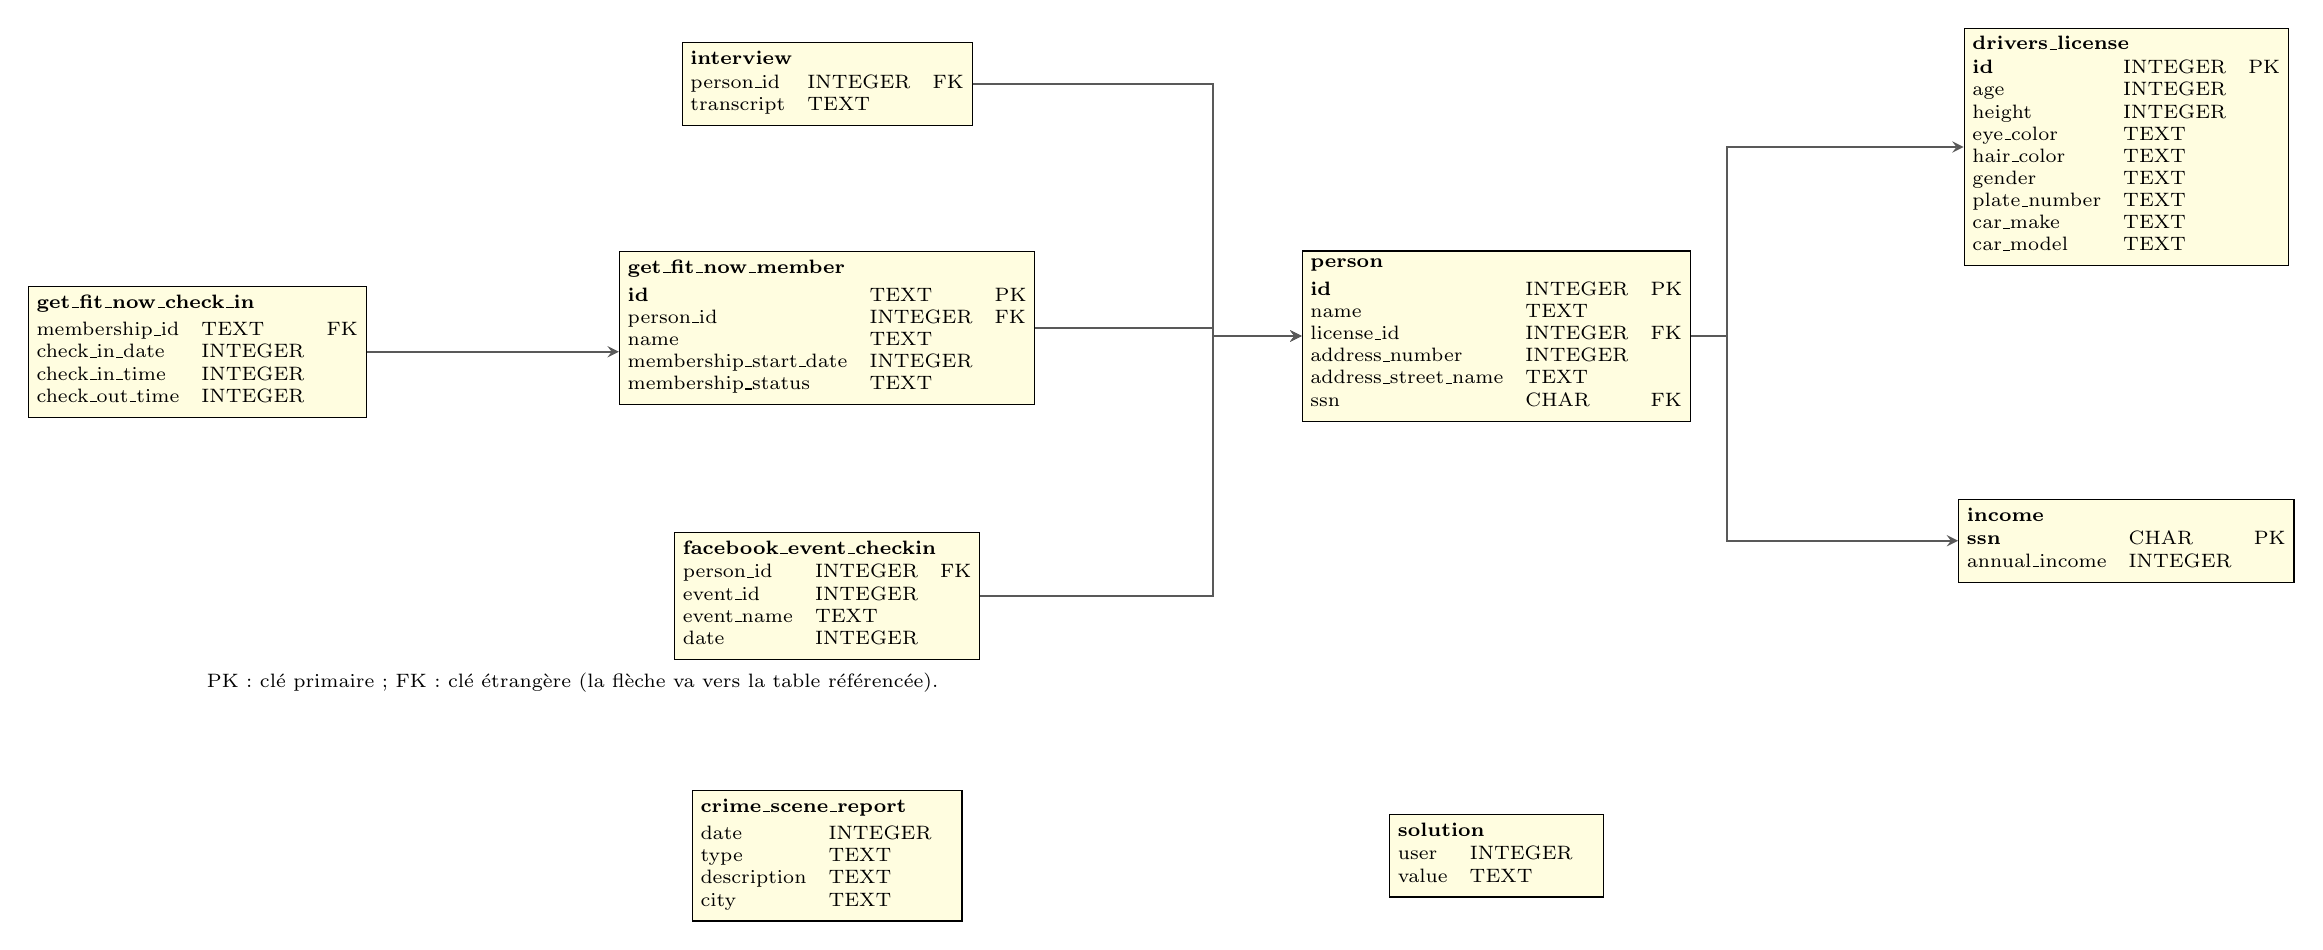
\begin{tikzpicture}[x=1cm,y=1cm,tbl/.style={draw,fill=yellow!12,inner sep=3pt,font=\scriptsize,align=left},fk/.style={->,>=stealth,thick,gray!70!black}]
\node[tbl] (get_fit_now_check_in) at (0.0,0.0) {\textbf{get\_fit\_now\_check\_in}\\[2pt]\begin{tabular}{@{}l@{\quad}l@{\quad}l@{}}
membership\_id & TEXT & FK\\
check\_in\_date & INTEGER & \\
check\_in\_time & INTEGER & \\
check\_out\_time & INTEGER & \\
\end{tabular}};
\node[tbl] (interview) at (8.0,3.4) {\textbf{interview}\\[2pt]\begin{tabular}{@{}l@{\quad}l@{\quad}l@{}}
person\_id & INTEGER & FK\\
transcript & TEXT & \\
\end{tabular}};
\node[tbl] (get_fit_now_member) at (8.0,0.3) {\textbf{get\_fit\_now\_member}\\[2pt]\begin{tabular}{@{}l@{\quad}l@{\quad}l@{}}
\textbf{id} & TEXT & PK\\
person\_id & INTEGER & FK\\
name & TEXT & \\
membership\_start\_date & INTEGER & \\
membership\_status & TEXT & \\
\end{tabular}};
\node[tbl] (facebook_event_checkin) at (8.0,-3.1) {\textbf{facebook\_event\_checkin}\\[2pt]\begin{tabular}{@{}l@{\quad}l@{\quad}l@{}}
person\_id & INTEGER & FK\\
event\_id & INTEGER & \\
event\_name & TEXT & \\
date & INTEGER & \\
\end{tabular}};
\node[tbl] (person) at (16.5,0.2) {\textbf{person}\\[2pt]\begin{tabular}{@{}l@{\quad}l@{\quad}l@{}}
\textbf{id} & INTEGER & PK\\
name & TEXT & \\
license\_id & INTEGER & FK\\
address\_number & INTEGER & \\
address\_street\_name & TEXT & \\
ssn & CHAR & FK\\
\end{tabular}};
\node[tbl] (drivers_license) at (24.5,2.6) {\textbf{drivers\_license}\\[2pt]\begin{tabular}{@{}l@{\quad}l@{\quad}l@{}}
\textbf{id} & INTEGER & PK\\
age & INTEGER & \\
height & INTEGER & \\
eye\_color & TEXT & \\
hair\_color & TEXT & \\
gender & TEXT & \\
plate\_number & TEXT & \\
car\_make & TEXT & \\
car\_model & TEXT & \\
\end{tabular}};
\node[tbl] (income) at (24.5,-2.4) {\textbf{income}\\[2pt]\begin{tabular}{@{}l@{\quad}l@{\quad}l@{}}
\textbf{ssn} & CHAR & PK\\
annual\_income & INTEGER & \\
\end{tabular}};
\node[tbl] (crime_scene_report) at (8.0,-6.4) {\textbf{crime\_scene\_report}\\[2pt]\begin{tabular}{@{}l@{\quad}l@{\quad}l@{}}
date & INTEGER & \\
type & TEXT & \\
description & TEXT & \\
city & TEXT & \\
\end{tabular}};
\node[tbl] (solution) at (16.5,-6.4) {\textbf{solution}\\[2pt]\begin{tabular}{@{}l@{\quad}l@{\quad}l@{}}
user & INTEGER & \\
value & TEXT & \\
\end{tabular}};
\draw[fk] (get_fit_now_check_in.east) -- (get_fit_now_member.west|-get_fit_now_check_in.east);
\draw[fk] (get_fit_now_member.east) -- (12.9,0 |- get_fit_now_member.east) |- (person.west);
\draw[fk] (interview.east) -- (12.9,0 |- interview.east) |- (person.west);
\draw[fk] (facebook_event_checkin.east) -- (12.9,0 |- facebook_event_checkin.east) |- (person.west);
\draw[fk] (person.east) -- ++(0.45,0) |- (drivers_license.west);
\draw[fk] (person.east) -- ++(0.45,0) |- (income.west);
\node[font=\scriptsize,anchor=west] at (0,-4.2) {PK : clé primaire ; FK : clé étrangère (la flèche va vers la table référencée).};
\end{tikzpicture}}
    \captionsetup{labelformat=empty}
    \caption{Schéma relationnel de la base de données SQL Murder Mystery.}
    \label{fig:SQLmystery-table}
\end{figure}
\end{landscape}